
In the next chapters, a numerical simulation tool enabling the characterization of existing breast compression techniques in terms of patient comfort is developed. 
 The latter would serve to build an optimal compression paddle considering the patient experience during mammography.  
 
In this purpose, MR images of two subjects are used to create patient specific finite elements breast models. The mechanical behavior of soft tissues under compression is computed for both subjects and for both paddle designs. The perceived pain for a given paddle design is quantitatively characterized by contact pressure, internal stress and strain distributions. After compression, three sets of macrocalcifications are inserted into breast volumes. The latter are then subject to a Monte-Carlo based simulation (CatSim) enabling to simulate the image acquisition of the compressed breast with a mammography system. Then, the diagnosis quality is assessed by measuring the signal-difference-to-noise-ratio (SDNR), signal-to-noise-ratio (SNR) and the average glandular dose (AGD). 

\clearpage


\section{Breast compression modeling}

\subsection{FE modeling of compression paddles}
In this study only standard paddle generally used for regular screening will be considered. Only one paddle geometry was considered based on the technical specifications from a Senographe PristinaTM mammography unit (GE-Healthcare, Buc, France). The paddle flexibility due to the material properties was neglected. The SRP was therefore defined as a fully rigid body with only one translational degree of freedom in the downwards direction. For the SFP, a rotation around the longitudinal axis is added. An additional degree of freedom was modeled using a rotational-only joint type of element.

The joint stiffness was computed by fitting the force-deflection curve of a flex paddle from a Senographe PristinaTM unit. A rigid plate was fixed at the external edge between the bucky and the SFP (Figure \ref{fig:deflectionangle}.a). To ensure the paddle rotation about the $Oy$ axis only, the rigid plate was chosen to have the same length (in $Oy$ direction) as the compression paddle. The deflection angle was measured using a digital inclinometre ($\pm0.1deg$ accuracy). The paddle was lowered progressively, such as the deflection angle was incremented by about $0.5 deg$, until the maximal recommended compression force is reached ($F=200N$). At each step, the compression force was read from the calibrated mammograph unit. The experiment was repeated 3 times. The relation between the mean compression force and the deflection angle is shown in Figure \ref{fig:deflectionangle}.b. The estimated second degree polinomial was used to define the joint stiffness for the FE analysis.

\begin{figure}[!h]
\centering
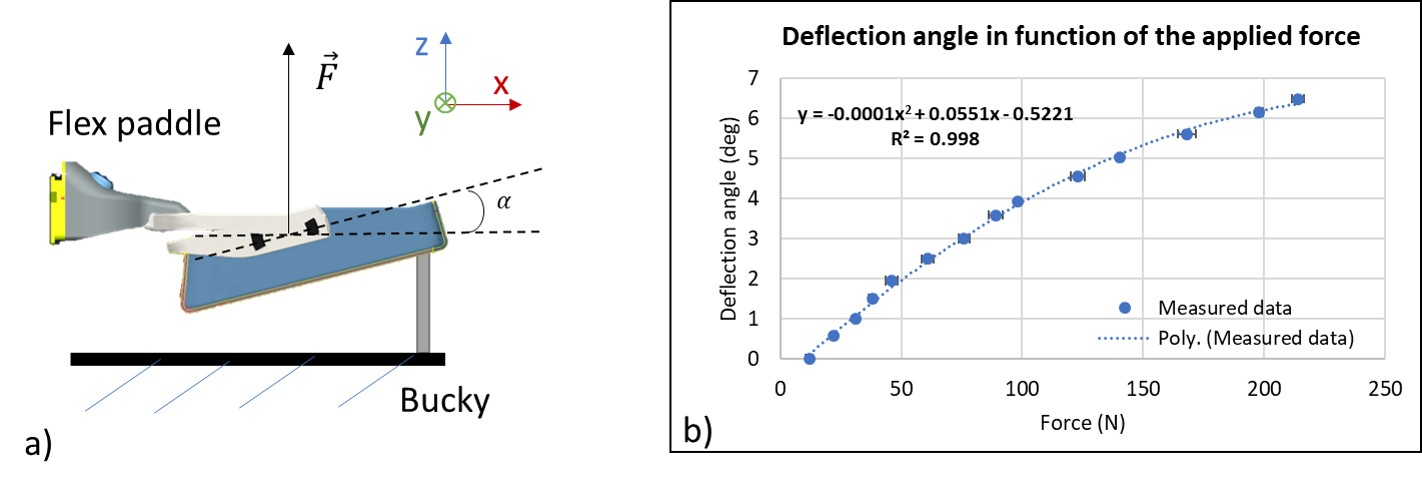
\includegraphics[width=0.9\textwidth,keepaspectratio]{figures/deflectionAngle.jpg} 
\caption{ a) Experiment set-up, b) Deflection angle in function on the applied force }\label{fig:deflectionangle}
\end{figure}

 
\subsection{Breast compression mechanics}

The compression of small breasts may be complex. Sometimes the technologist have to hold the breast between the bucky and the  paddle until the compression force is high enough to preclude breast from sliding outside of the compression area. These difficulties are also meet in a simulation framework, all the more so because the technologist breast manipulation is not reproduced. To facilitate the compression task, the following breast compression tests are made on the geometry of the second volunteer.

When breast is compressed the gravity induced tissues pre-stresses can be neglected when compared to the compression induced stresses \citep{han_development_2012, ruiter_model_based_2006, sturgeon_finite_element_2016}. In a clinical framework, woman breast is compressed only in a up-right or prone body position. Therefore, for this section, the prone breast configuration was used as reference configuration by neglecting the tissues internal pre-stresses dues to gravity loading.

Previously developed biomechanical model is implemented  using the breast geometry of the second volunteer. Because of the large computation time the constitutive parameters were not addapted to the volunteer-specific mechanical behavior. Their values were taken from the literature \citep{han_nonlinear_2014,rajagopal_modelling_2007,gefen_mechanics_2007}, and were chosen the following $\lambda_{breast}=0.5 kPa$, $\lambda_{muscle}= 10kPa$, $\lambda_{skin}=10$, $\lambda_{fascia}= 160kPa$.    

To simulate the cranio-caudal incidence, the bucky is positioned at the inframammary ligament level while the paddle compresses the breast by a downward movement. The compression is stopped then the target breast thickness is reached. The target thickness is given by the data  obtained during the volunteers last mammogram (Table \ref{tab:forceandthichnessdata}). The Figure \ref{fig:thicknessforcerelationNH}) shows the breast thickness as function of the applied force for the flex and the rigid paddles. The breast thickness is considered constant then compressing with the SRP, and is equal to the mean thickness when compressing with the SFP. 
 
\begin{figure}[!h]
\centering
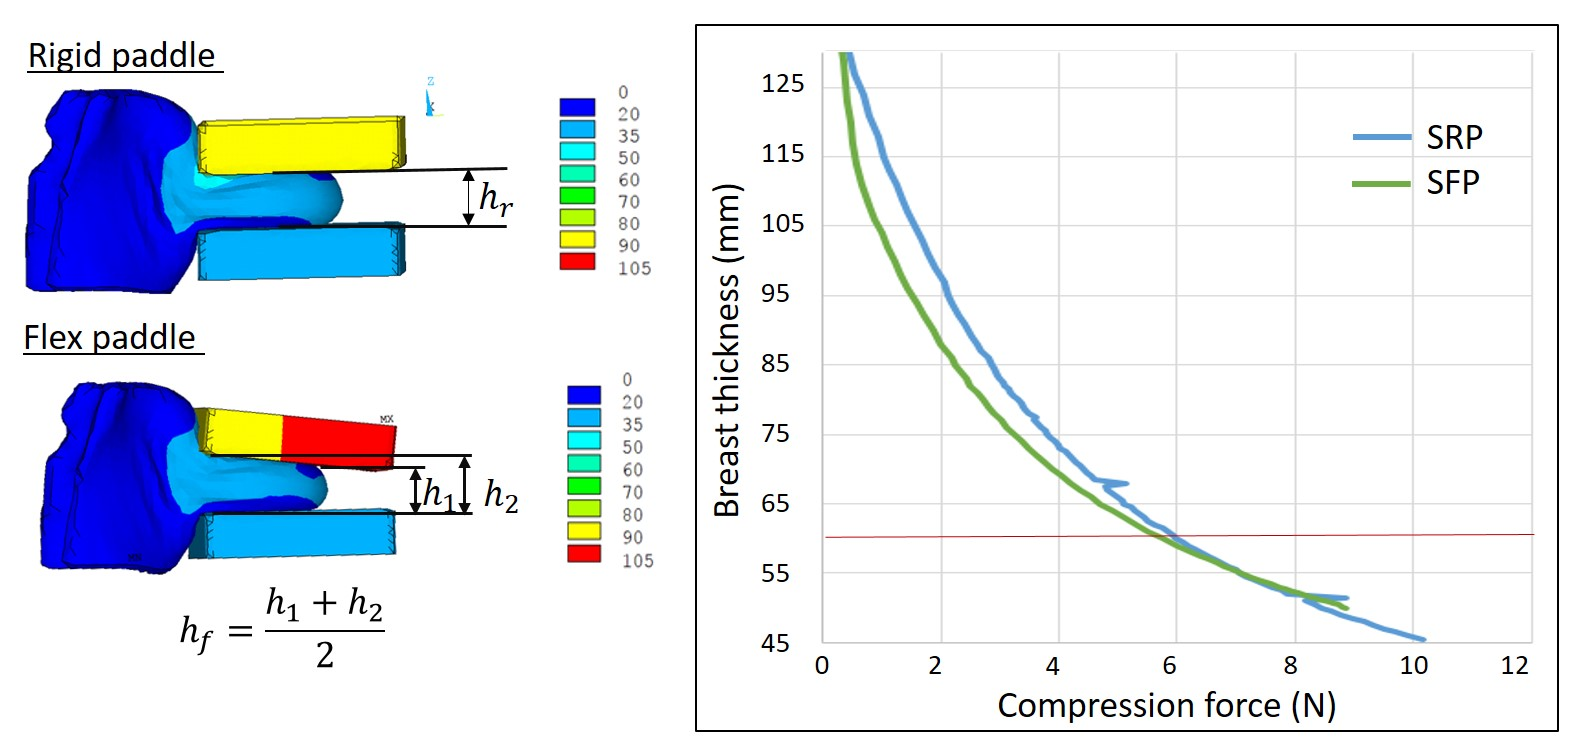
\includegraphics[width=0.9\textwidth,keepaspectratio]{figures/compressionforceNH.jpg} 
\caption{Breast flattening curve as function of the applied force for a Neo-Hookean strain energy function. SRP - standard rigid paddle, SFP -standard flex paddle}\label{fig:thicknessforcerelationNH}
\end{figure}

One can see that, the total compression force at the target breast thickness ($50mm$) is about 10 times lower then the force measured during the volunteer's last mammography ($6N$ versus $94.8N$). Several compression were tested (paddle closer to the juxtathoracic area, frictional contact with different friction coefficient) without significantly increasing the compression force. 

An analysis of the literature revealed that the constitutive parameters used for modeling the breast compression are higher than the ones used for modeling the breast deformation under gravity loading.  \cite{sturgeon_finite_element_2016}  have modeled the tissues deformation under compression considering the initial shear moduli for the Neo-Hookean potential function equal to $\mu_{skin} = 88kPa$, $\mu_{adipose} = 1kPa$ and $\mu_{glandular}= 10kPa$. In the same time, \cite{han_nonlinear_2014} estimated the initial shear modulus of 5 subject giving the best match between the prone and supine breast geometries. According to the authors, the constitutive parameters ranges were as following  $\mu_{adipose}=0.61-3.49 kPa$, $\mu_{glandular}=0.72-4.35$ and $\mu_{skin} = 2.47 - 5.78 $. 

When the curve behavior is compared to the ones given by \cite{de_pain_2015} 


\section{Image acquisition simulation }
\subsection{Microcalcifications}
Microcalcifications $(\mu calc)$ were simulated as surface mesh objects. Round-shaped microcalcifications were considered. Spheres were first simulated. Then, to add irregularities and randomness to the simulated $(\mu calc)$ , the sphere surface of each $(\mu calc)$  was randomly deformed. The deformation consisted of two steps. First, the sphere surface was slightly deformed to a random ellipsoid along three randomly chosen axes, with maximum deformation magnitude set to five percent of the $(\mu calc)$  diameter. Then the surface meshes were modified according to a stochastic Perlin noise to create irregularities. The Perlin noise deformation was done by locally displacing the vertices of a surface mesh in directions perpendicular to the mesh face. The displacement magnitude was set to $20 \mu m$.
Microcalcifications with two diameters, $200 \mu m$ and $300 \mu m$, were considered to account for a realistic range of $(\mu calc)$ sizes as seen in clinical practice.

Microcalcifications with x-ray attenuation properties corresponding to the attenuation of aluminum (Al) at 22 $keV$ and with the same volumetric mass density as Al, i.e. 2.72 $kgm^{−3}$, were designed. 
The choice of 22 $keV$ corresponded to the photon energy of the x-ray source used in our study. Al is less attenuating than the minerals composing real μcalcs which contain calcium carbonate, calcium oxalate or apatite. This is realistic since in real $(\mu calc)$, the minerals are embedded in a protein matrix; therefore the attenuation of a $(\mu calc)$ is lower than when considering only the minerals.

Physical characteristics of the imaging system were modeled as follows. A simplified
mono-energetic x-ray source was used. The photon energy level was set to 22 keV, this is equivalent to the effective x-ray energy of a 34 kVp Rhodium (Rh)/Silver (Ag) target/filter spectrum used for imaging a 50mm compressed breast. An ideal point source focal-spot was used. In order to simulate the detector unsharpness, a modulation transfer function empirically measured from the reference system was used by the simulator. X-ray scatter from the test object was not considered. Only Poisson x-ray noise was added and the electronic noise was not modeled.
A calibration was performed to match the signal-to-noise ratio (SNR) in simulated images with the SNR obtained in experimentally acquired images using the GE Senographe
Pristina system with automatic optimization of parameters (AOP).

To assess the impact of breast compression on image quality, we inserted a set of microcalcifications into each compressed breast volume. The smallest breast volume contains 21 microcalcifications arranged in a matrix of 7 rows and 3 columns (Figure 4a). The largest breast volume contains 56 microcalcifications arranged in a matrix of 7 rows and 8 columns. The matrix of calcifications is parallel with the entrance surface of the image receptor and positioned at the breast mid thickness (Figure 4b). The distance between two consecutive columns or rows is 10mm. We assumed a uniform breast-equivalent material composed of glandular/adipose tissue with a 20/80 ratio. A mammogram was simulated using typical clinical acquisition parameters obtained with the standard automatic optimization of parameters (AOP) mode. Two simulations were performed with microcalcifications of 0.2 mm and 0.3mm in diameter.

\begin{figure}[!h]
\centering
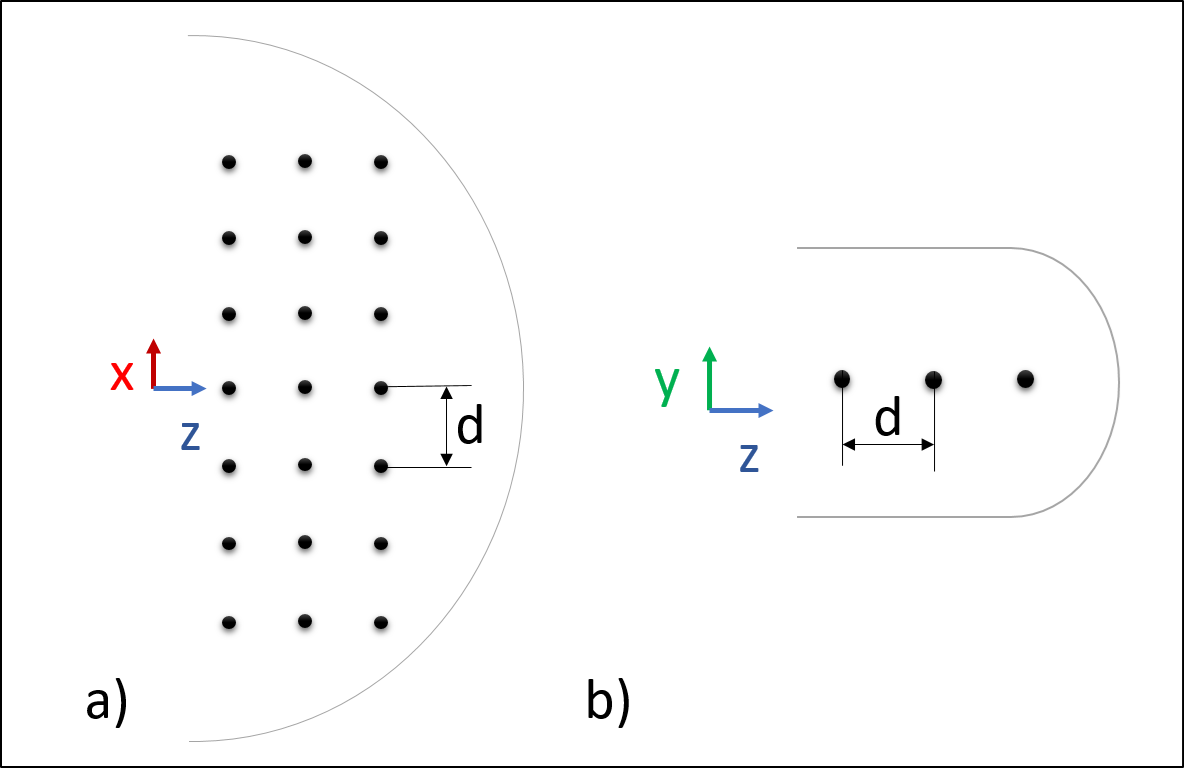
\includegraphics[width=0.5\textwidth,keepaspectratio]{figures/microcalcifications.png} 
\caption{Microclcification distribution over the smallest breast volume $(d=10mm)$: a)axial view, b) sagittal view.}\label{fig:compressionpaddles}
\end{figure}

\subsection{Simulation of digital images}

Topology of the FFDM image acquisition was modeled as follows. The source-toimage
distance (SID) was set to 660mm. The detector size was set to 239.4mm in the
x-axis direction and 286mm in the y-axis direction. Isotropic detector pixels with size of
0.1mm were simulated. Position of the x-ray source was modeled such that its projection
along the z axis onto the detector plane falls exactly at the midpoint of the detector’s left
edge. The bucky and the compression paddle were modeled as two planes parallel to the
detector.


\section{Compression quality metrics}\label{section:compressionqualitymetrics}
\subsection{Patient comfort}

Today, the pain estimation and quantification still remains an open question. During mammography, the perceived pain, or it's interpretation, may depend on the social status, pain history or psychological condition of the patient. But can also depend on the physical parameters as the compression force, amount of deformation or pressure on the skin surface. In clinical studies the patient comfort is studied using pain scales, the repetability of such methods are questionable, because is based on the patient own interpretation and expertise. More quantitative measures such as pupil dilatation, heart rate are interesting in assessing the patient comfort, however they may indicate not only the pain but also the fear of  pain.        

In this work, only the physical pain associated with tissues deformation was considered. In this scope, the maximal stain and stress intensities as well as the maximal pressure intensity at the contact surface between the breast and the compression paddle were chosen as pain quantifiers. Their distribution over the breast volume were obtained from FE simulation of breast compression and  were analyzed in order to compare the patient experience between two distinct compressions. 

\subsection{Image quality }\label{section:averagegalndulardose}
 The signal-difference-tonoise ratio (SDNR) per pixel of these microcalcifications was measured. Additionally, the signal-to-noise ratio (SNR) was computed on the same pixels excluding the microcalcifications.  




\subsection{ Average glandular dose}
The average glandular dose (AGD) was derived using the approach proposed by Dance et al12 regardless the paddle type.  In practice, it is very difficult to accurately measure the exact breast thickness. Thus, the nominal breast thickness was used to compute conversions factors which relate measurements of incident air kerma to the delivered mean glandular dose.

\section{Results}\label{section:breastcompressionevaluation}
With a rigid paddle, the breast under compression presents a nearly uniform thickness all over the contact surface. Contrariwise, with a flex paddle, the compressed breast thickness decreases quasi linearly from the chest wall to the nipple. Flex paddles are used to better conform the breast contours and thereby to improve compression. However, Broeders and collegues11 have shown that such compression paddle may decrease the diagnostic quality of mammograms as the breast tissues may be pushed out to the chest wall resulting in less retro-glandular tissue visible on the image. 

The force versus breast thickness curves are plotted in Figure 5 for both volunteers with the rigid and flex paddles. We observed a nominal compression thickness roughly equals for both paddles. The resulting internal stress and strain distributions, as well as contact pressure maps were derived at compressive forces of 22 N for the first volunteer (Figure \ref{fig:subject1_compressionResults}) and 95 N for the second one (Figure \ref{fig:subject2_compressionResults}).

\begin{figure}[!h]
\centering
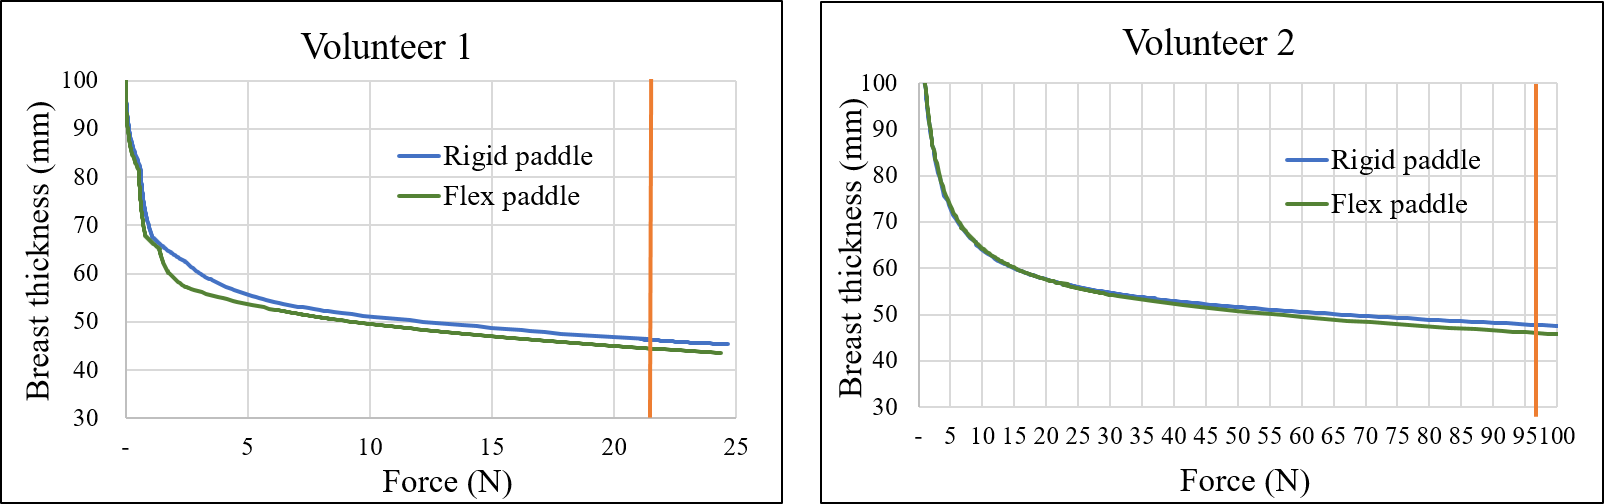
\includegraphics[width=0.9\textwidth,keepaspectratio]{figures/forceThicknessResults.png} 
\caption{Resulting breast thickness for a given compression force}\label{fig:forceThicknessResults}
\end{figure}

As concerns the small breast volume (Figure \ref{fig:subject1_compressionResults}), there is no significant difference between FCP and RCP in pressure distribution over the skin surface or in internal stress/strain intensity distributions. For both compression paddles, high pressure at the skin surface is concentrated in the juxtathoracic region with a maximum pressure of 77.7 kPa. Several clinical studies11,13 sustained this result of no significant difference in experienced pain when using FCP or RCP. In addition, the FE simulations confirm that in small breasts the paddle tilt is too small to impact the tissues compression in the middle part of the breast. 
FCP applied on large breast volumes (Figure \ref{fig:subject2_compressionResults}) results in significantly lower intensities of pressure at the skin surface in contact with the compression paddle, with a maximal pressure of 37 kPa, compared to 56 kPa when using RCP. No significant difference in the measured maximal intensities of strain and stress was observed, however strain and stress distribution patterns are different. When the breast is compressed with a rigid paddle, maximal strain and stress are concentrated in the retromammary space and decrease considerably toward the nipple. When a flex paddle is used, stress and strain are more uniformly distributed over the breast volume with the highest values in the middle third of the breast.
The areal pressure distribution patterns has already been demonstrated in the work by Dustler and collegues13. The authors have studied the pressure distribution patterns of 103 women undergoing breast compression with a rigid paddle at different compression levels. Four groups have been differentiated: a) skin pressure widespread over the breast (29\%); b) skin pressure concentrated on the central part of the breast (8\%); c) skin pressure concentrated on the juxtathoracic region (16\%); d) skin pressure concentrated along a narrow zone at the juxtathoracic region (26\%).  The pressure distribution patterns observed for our first and second volunteers correspond to the group d and a respectively.


\begin{figure}[!h]
\centering
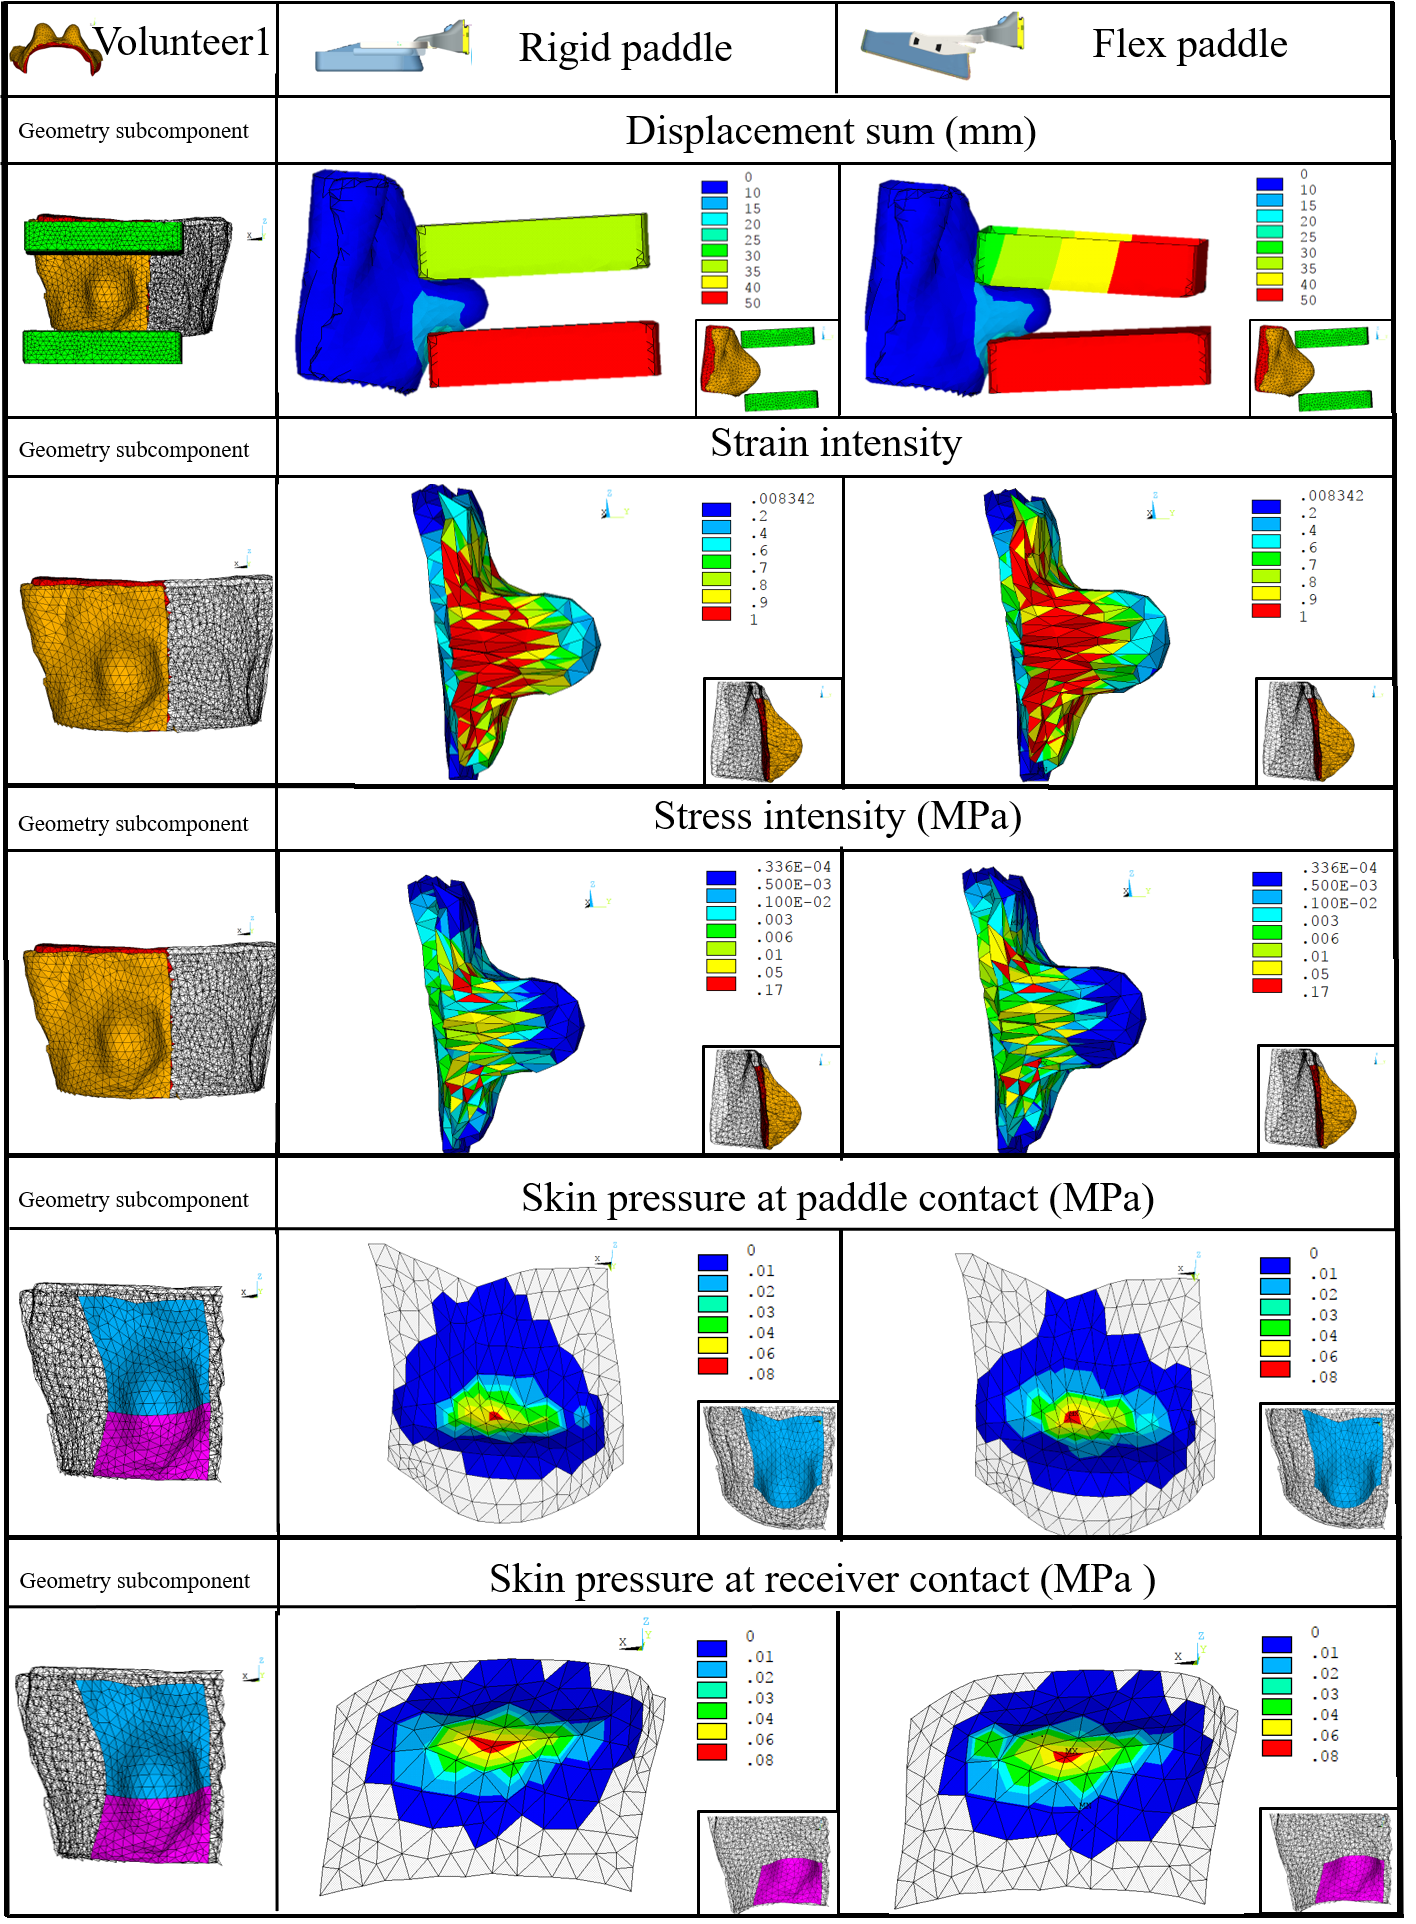
\includegraphics[width=0.95\textwidth,keepaspectratio]{figures/subject1_compressionResults.png} 
\caption{Stress, strain and contact pressure distribution for the first subject}\label{fig:subject1_compressionResults}
\end{figure}

\begin{figure}[!h]
\centering
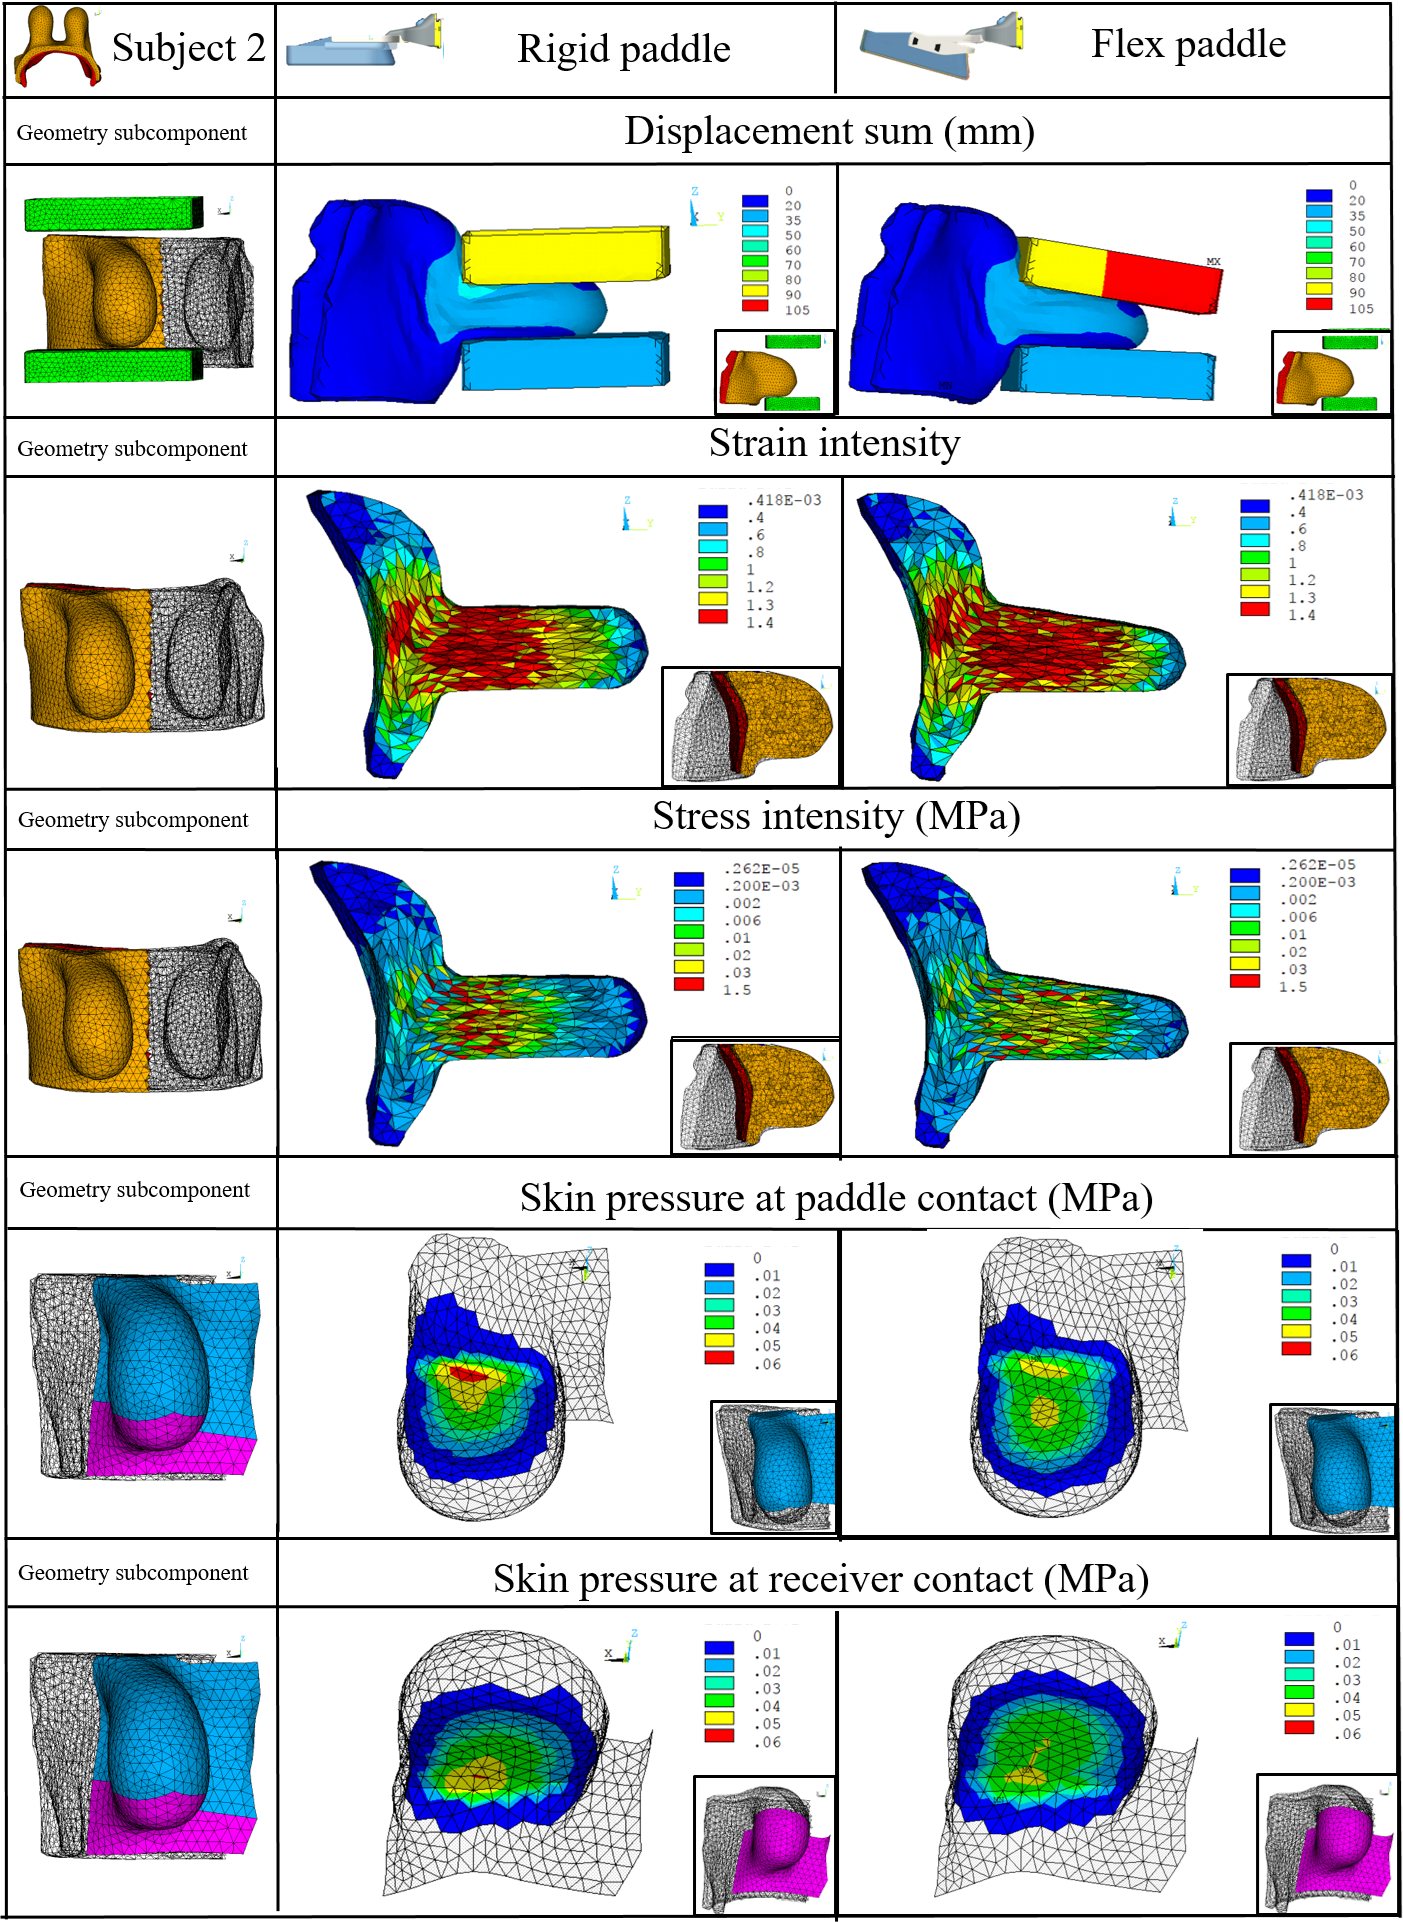
\includegraphics[width=0.95\textwidth,keepaspectratio]{figures/subject2_compressionResults.png} 
\caption{Stress, strain and contact pressure distribution for the second subject}\label{fig:subject2_compressionResults}
\end{figure}

The nominal breast thickness may vary by about 2mm between rigid and flex paddle for both volunteers (Table \ref{fig:table_compression_results}). Accordingly, no significant difference was found between the estimated AGD, while a dose reduction of 2\% for the smaller breast and 4\% for larger breast was observed.

\begin{figure}[!h]
\centering
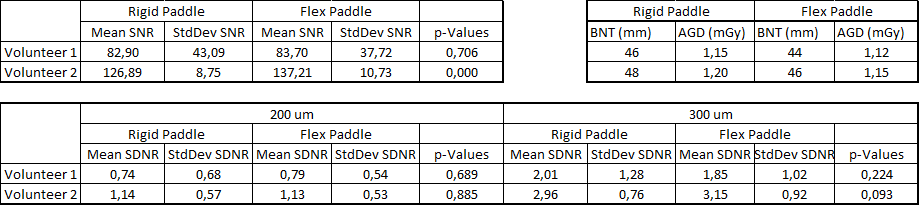
\includegraphics[width=\textwidth,keepaspectratio]{figures/table_compression_results.png} 
\caption{Breast nominal thickness (BNT), average glandular dose (AGD), signal-to-noise-ratio (SNR) and signal-difference-to-noise (SDNR) for both volunteers and both compression paddle types}\label{fig:table_compression_results}
\end{figure}

The SNR and SDNR have been estimated and compared between flex and rigid paddles. When using a flex paddle instead of a rigid paddle on the largest breast (volunteer 2), we observe a statistically significantly higher SNR. The same trend is observed on SDNR for both 200 and 300 µm microcalcifications, while not statistically significant. We did not observe any statistically significant difference in SNR or SDNR for microcalcification of any size when considering the compression of the smallest breast by a rigid or a flex paddle. Therefore, despite a breast thickness varying linearly from chest wall to nipple when the flex compression paddle is used, the image quality is preserved or improves compared to the image quality obtained with the rigid compression paddle.

\section{Discussions and conclusion}\label{section:compressionfem:conclusion}

Breast compression with flex and rigid paddle have been simulated using the finite elements theory applied to segmented MRI images acquired on 2 volunteers under different geometries. Appling the Gent form of strain-energy potential, instead of the Neo-Hookean form, allowed to obtain compression force magnitudes comparable with the real subject data.  
After simulating the breast compression, the SDNR of microcalcifications and the AGD, delivered during the acquisition of the corresponding simulated mammography, have been computed. The simulations have been repeated for two different breast volumes (cup sizes A and F) with a rigid and a flex paddle. The four configurations have been analyzed to compare patient perceived pain (measured as strain and stress) and image quality (measured as SNR, SDNR and AGD). The results of our simulations indicate that, for the smallest breast, there is no significant difference for the patient perceived pain when using the rigid or the flex paddle. The shape of the breast under compression does not present significant changes between the two paddle designs. We did not observe any statistically significant difference in SNR or SDNR for microcalcification of any size when considering the compression of the smallest breast by a rigid or a flex paddle. Therefore, our results suggest that using a flex paddle should not significantly impact image quality and delivered dose in small breasts, and should not reduce significantly the perceived pain.   
For the largest breast, our simulations indicate that using a flex paddle may reduce the maximal pressure intensity on the skin surface by about 30\% compared to the rigid paddle. The tissues deformation is more uniformly distributed inside the breast volume, and the highest deformation is occurring in the middle breast region corresponding to the supposed location of dense tissues. Moreover, our simulations have shown that flex paddle have no significant impact on the average glandular dose and improves image quality compared to the rigid paddle. 
In conclusion, our simulations confirm that using the flex paddle used for breast compression may improve the patient comfort without affecting the image quality and the delivered average glandular dose. Moreover, despite a breast thickness varying linearly from chest wall to nipple, when a flex compression paddle is used on large breasts, the image quality seems to be preserved or improved compared to the image quality obtained with a rigid compression paddle
